\setbeamercolor{background canvas}{bg=fitblue}
\begin{frame}
\frametitle{Projection / Projekce}
\begin{center}
\Huge {\color{white}Projection / Projekce}
\end{center}
\end{frame}
\setbeamercolor{background canvas}{bg=white}

\begin{frame}\frametitle{Orthographics projection / Ortogonální projekce}
In case of orthographics projection, view-volume has shape of a block.
There se six parameters: l,r,b,t,n,f (left, right, bottom, top, near, far).\\
U ortogonální projekce je tvar pohledového tělesa kvádr.
Kvádr má 6 parametrů: l (left),r (right),b (bottom),t (top),n (near),f (far).
\begin{figure}[htb]
	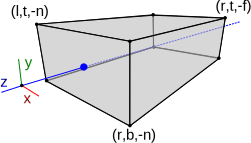
\includegraphics[height=4cm,keepaspectratio]{pics/projection/ortho}
	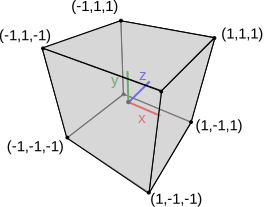
\includegraphics[height=4cm,keepaspectratio]{pics/projection/ndc}
\end{figure}
\end{frame}

\begin{frame}
\frametitle{Orthographic projection / Ortogonální projekce}
\begin{figure}[htb]
	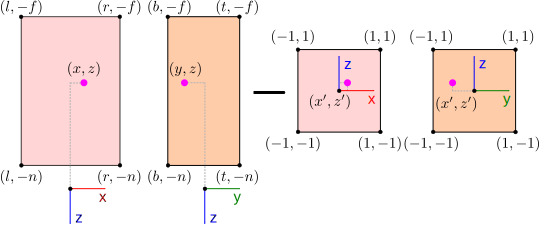
\includegraphics[height=4cm,keepaspectratio]{pics/projection/fromortho}
\end{figure}
\end{frame}

\begin{frame}
\frametitle{Orthographic projection / Ortogonální projekce}
\begin{multicols}{3}
{\tiny
\begin{eqnarray*}
	x &\in& [l,r] \\
	x-l &\in& [0,r-l] \\
	\frac{x-l}{r-l} &\in& [0,1] \\
	2 \frac{x-l}{r-l} &\in& [0,2] \\
	2 \frac{x-l}{r-l}-1 &\in& [-1,1]\\
	2 \frac{x-l}{r-l}- \frac{r-l}{r-l} &=& x'\\
	\frac{2}{r-l}x - \frac{r+l}{r-l} &=& x'
\end{eqnarray*}
}
\vfill
{\tiny
\begin{eqnarray*}
	y &\in& [b,t] \\
	y-b &\in& [0,t-b] \\
	\frac{y-b}{t-b} &\in& [0,1] \\
	2 \frac{y-b}{t-b} &\in& [0,2] \\
	2 \frac{y-b}{t-b}-1 &\in& [-1,1]\\
	2 \frac{y-b}{t-b}- \frac{t-b}{t-b} &=& y'\\
	\frac{2}{t-b}y - \frac{t+b}{t-b} &=& y'
\end{eqnarray*}
}
\vfill
{\tiny
\begin{eqnarray*}
	z &\in& [-n,-f] \\
	z+n &\in& [0,n-f] \\
	\frac{z+n}{n-f} &\in& [0,1] \\
	2 \frac{z+n}{n-f} &\in& [0,2] \\
	2 \frac{z+n}{n-f}-1 &\in& [-1,1]\\
	2 \frac{z+n}{n-f}- \frac{n-f}{n-f} &=& z'\\
	\frac{-2}{f-n}z + \frac{f+n}{f-n} &=& z'
\end{eqnarray*}
}
\end{multicols}

\end{frame}

\begin{frame}
\frametitle{Orthographic projection / Ortogonální projekce}
$$
\left[
\begin{array}{cccc} 
a_{1,1} & a_{1,2} & a_{1,3} & a_{1,4} \\
a_{2,1} & a_{2,2} & a_{2,3} & a_{2,4} \\
a_{3,1} & a_{3,2} & a_{3,3} & a_{3,4} \\
a_{4,1} & a_{4,2} & a_{4,3} & a_{4,4}
\end{array}
\right]
\cdot
\left[
\begin{array}{c}
x \\
y \\
z \\
1
\end{array}
\right]
=
\left[
\begin{array}{c} 
x' \\
y' \\
z' \\
1
\end{array}
\right]
=
\left[
\begin{array}{c} 
\frac{2}{r-l}x - \frac{r+l}{r-l}\\
\frac{2}{t-b}y - \frac{t+b}{t-b}\\
\frac{-2}{f-n}z + \frac{f+n}{f-n}\\
1
\end{array}
\right]
$$

$$
\left[
\begin{array}{cccc} 
\frac{2}{r-l} & 0             & 0              & -\frac{r+l}{r-l} \\
0             & \frac{2}{t-b} & 0              & -\frac{t+b}{t-b} \\
0             & 0             & \frac{-2}{f-n} & \frac{f+n}{f-n} \\
0             & 0             & 0              & 1
\end{array}
\right]
\cdot
\left[
\begin{array}{c}
x \\
y \\
z \\
1
\end{array}
\right]
=
\left[
\begin{array}{c} 
x' \\
y' \\
z' \\
1
\end{array}
\right]
$$
\end{frame}

\begin{frame}
\frametitle{Perspective projection / Perspektivní projekce}
View-volume of perspective projection has a shape of frustum - view-frustum.
There are also six parameters: l,r,b,t,n,f.\\
U perspektivní projekce je tvar pohledového tělesa komolý jehlan.
Stejně jako u Ortogonální projekce má 6 parametrů: l (left),r (right),b (bottom),t (top),n (near),f (far).
Jehlan je umístěn relativně ke středu systému.
\begin{figure}[htb]
	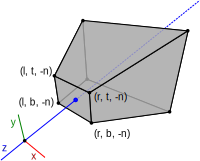
\includegraphics[height=4cm,keepaspectratio]{pics/projection/pers}
	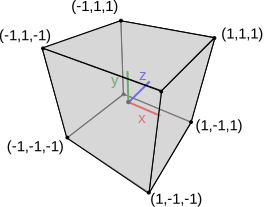
\includegraphics[height=4cm,keepaspectratio]{pics/projection/ndc}
\end{figure}
\end{frame}

\begin{frame}
\frametitle{Perspective projection / Perspektivní projekce}
\begin{figure}[htb]
	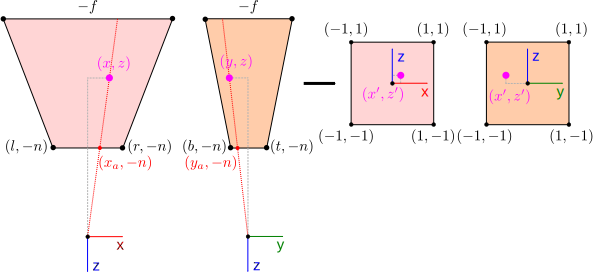
\includegraphics[height=5cm,keepaspectratio]{pics/projection/frompers}
\end{figure}
\end{frame}

\begin{frame}
\frametitle{Perspective projection / Perspektivní projekce}
\begin{multicols}{2}
{\tiny
\begin{eqnarray*}
	\frac{x_a}{-n} &=& \frac{x}{z} \\
	x_a &=& \frac{-nx}{z} \\
	x_a &\in& [l,r] \\
	x_a-l &\in& [0,r-l] \\
	\frac{x_a-l}{r-l} &\in& [0,1] \\
	2\frac{x_a-l}{r-l}-1 &\in& [-1,1] \\
	\frac{2}{r-l}x_a-\frac{r+l}{r-l} &=& x'\\
	\frac{-2n}{r-l} \frac{x}{z} - \frac{r+l}{r-l} &=& x'
\end{eqnarray*}
\begin{equation}
\label{eq:persx}
\frac{-2n}{r-l} \frac{x}{z} - \frac{r+l}{r-l} = x'
\end{equation}
}
\vfill
{\tiny
\begin{eqnarray*}
	\frac{y_a}{-n} &=& \frac{y}{z} \\
	y_a &=& \frac{-ny}{z} \\
	y_a &\in& [b,t] \\
	y_a-b &\in& [0,t-b] \\
	\frac{y_a-b}{t-b} &\in& [0,1] \\
	2\frac{y_a-b}{t-b}-1 &\in& [-1,1] \\
	\frac{2}{t-b}y_a-\frac{t+b}{t-b} &=& y'\\
	\frac{-2n}{t-b} \frac{y}{z} - \frac{t+b}{t-b} &=& y'
\end{eqnarray*}
\begin{equation}
\label{eq:persy}
\frac{-2n}{t-b} \frac{y}{z} - \frac{t+b}{t-b} = y'
\end{equation}
}
\end{multicols}

\end{frame}

\begin{frame}
\frametitle{Problem with z / Poblém se z}
\begin{multicols}{2}
{\tiny
\begin{eqnarray*}
	z &\in& [-n,-f] \\
	z+n &\in& [0,n-f] \\
	\frac{z+n}{n-f} &\in& [0,1] \\
	2\frac{z+n}{n-f}-1 &\in& [-1,1] \\
	\frac{2}{n-f}z+\frac{n+f}{n-f} &=& z'
\end{eqnarray*}
\begin{equation}
\label{eq:linz}
\frac{2}{n-f}z+\frac{n+f}{n-f} = z'
\end{equation}
}
\vfill
{\tiny
\begin{eqnarray*}
	\frac{1}{z} &\in& [-\frac{1}{n},-\frac{1}{f}] \\
	\frac{1}{z}+\frac{1}{n} &\in& [0,\frac{f-n}{nf}] \\
	\frac{nf}{f-n}\frac{1}{z}+\frac{f}{f-n} &\in& [0,1] \\
	\frac{2nf}{f-n}\frac{1}{z}+\frac{2f}{f-n}-1 &\in& [-1,1] \\
\end{eqnarray*}
\begin{equation}
\label{eq:persz}
\frac{2nf}{f-n}\frac{1}{z}+\frac{f+n}{f-n} = z'
\end{equation}
}
\end{multicols}

\end{frame}

\begin{frame}
\frametitle{Perspective projection / Perspektivní projekce}
{\tiny
\begin{equation}
\label{eq:swap}
\left[
\begin{array}{cccc} 
1 & 0 & 0 & 0 \\
0 & 1 & 0 & 0 \\
0 & 0 & 0 & 1 \\
0 & 0 & 1 & 0
\end{array}
\right]
\cdot
\left[
\begin{array}{c}
x \\
y \\
z \\
1
\end{array}
\right]
=
\left[
\begin{array}{c} 
x \\
y \\
1 \\
z
\end{array}
\right]
\end{equation}
}
\end{frame}

\begin{frame}
\frametitle{Perspective projection / Perspektivní projekce}
{\tiny
\begin{equation}
\label{eq:persmat1}
\left[
\begin{array}{cccc} 
-\frac{2n}{r-l} & 0               & 0                & -\frac{r+l}{r-l} \\
0               & -\frac{2n}{t-b} & 0                & -\frac{t+b}{t-b} \\
0               & 0               & \frac{2nf}{f-n} & \frac{f+n}{f-n} \\
0               & 0               & 0                & 1
\end{array}
\right]
\cdot
\left[
\begin{array}{c}
x \\
y \\
1 \\
z
\end{array}
\right]
=
\left[
\begin{array}{c}
x'\cdot z \\
y'\cdot z \\
z'\cdot z \\
z
\end{array}
\right]
\end{equation}
}
\end{frame}

\begin{frame}
\frametitle{Perspective projection / Perspektivní projekce}
The matrix after $z$ and $w$ replacement. / Matice pro prohození $z$ a $w$ složky v homogenních souřadnicích:
{\tiny
\begin{equation}
\left[
\begin{array}{cccc} 
-\frac{2n}{r-l} & 0               & 0               & -\frac{r+l}{r-l} \\
0               & -\frac{2n}{t-b} & 0               & -\frac{t+b}{t-b} \\
0               & 0               & \frac{2nf}{f-n} & \frac{f+n}{f-n} \\
0               & 0               & 0               & 1
\end{array}
\right]
\cdot
\left[
\begin{array}{cccc} 
1 & 0 & 0 & 0 \\
0 & 1 & 0 & 0 \\
0 & 0 & 0 & 1 \\
0 & 0 & 1 & 0
\end{array}
\right]
=
\left[
\begin{array}{cccc} 
-\frac{2n}{r-l} & 0               & -\frac{r+l}{r-l} & 0 \\
0               & -\frac{2n}{t-b} & -\frac{t+b}{t-b} & 0 \\
0               & 0               & \frac{f+n}{f-n} & \frac{2nf}{f-n} \\
0               & 0               & 1                & 0
\end{array}
\right]
\end{equation}
}
\end{frame}

\begin{frame}
\frametitle{Perspective projection / Perspektivní projekce}
{\tiny
\begin{equation}
\left[
\begin{array}{cccc} 
\frac{2n}{r-l} & 0               & \frac{r+l}{r-l} & 0 \\
0               & \frac{2n}{t-b} & \frac{t+b}{t-b} & 0 \\
0               & 0               & -\frac{f+n}{f-n} & -\frac{2nf}{f-n} \\
0               & 0               & -1                & 0
\end{array}
\right]
\cdot
\left[
\begin{array}{c}
x \\
y \\
z \\
1
\end{array}
\right]
=
\left[
\begin{array}{c}
-x'\cdot z \\
-y'\cdot z \\
-z'\cdot z \\
-z
\end{array}
\right]
\end{equation}
}
\end{frame}

